% !TeX TS-program = xelatex

\documentclass{beamer}
%Set the slide theme
%Change to meet your taste
% Madrid, Copenhagen, Berlin, ... works
% \usetheme{Madrid} 
\usetheme{metropolis}

\usepackage{xecolor}
\usepackage{amsmath}
%\usefonttheme[onlymath]{serif} %Change the math font
\usepackage{graphicx}
\graphicspath{{./images/}}
% \usepackage[nottoc]{tocbibind}
% \usepackage{wasysym}
 \usepackage{natbib}
\usepackage{doi}
 \usepackage{eso-pic}
 \usepackage{textpos}
\addtobeamertemplate{frametitle}{}{%
\begin{textblock*}{100mm}(-.88\textwidth,-1cm)

\includegraphics[width=1.cm]{arm_en}
\end{textblock*}}
\usepackage{xepersian}

\settextfont[Scale=1]{Yas}
% \setlatintextfont[Scale=1]{Times New Roman}
\setdigitfont{Yas}
\defpersianfont\titr{Yas}
\defpersianfont\nast{Yas}
% \bibliographystyle{asa-fa}
\bibliographystyle{chicago-fa.bst}
\renewcommand{\bibsection}{}
% {\bibliographystyle{./styles/iut-fa.bst}
% {\bibliographystyle{ieeetr-fa.bst}
% {\bibliographystyle{plainurl}
% {\bibliographystyle{plain-fa}
%---------------------------------------------------------------------------------
% Seetings to force Beamer works with Xepersian and RTL typesetting
%-------------------------------------------------------------------------------
%\raggedleft

% For right to left lists (itemize and enumerate)
\makeatletter
\newcommand{ \RTList}{\raggedleft\rightskip\@totalleftmargin} 
\makeatother
% Correct the bullet for RTL texts
\setbeamertemplate{itemize item}{\scriptsize\raise1.25pt%
 \hbox{\donotcoloroutermaths$\blacktriangleleft$}} 

% To force beamer use numbering in captions
\setbeamertemplate{caption}[numbered]{}% Number float-like environments

%  \logo{{
\includegraphics[width=1.4cm]{logo}}} 
% \newcommand{\nologo}{\setbeamertemplate{logo}{}}
\usebackgroundtemplate%
{%
    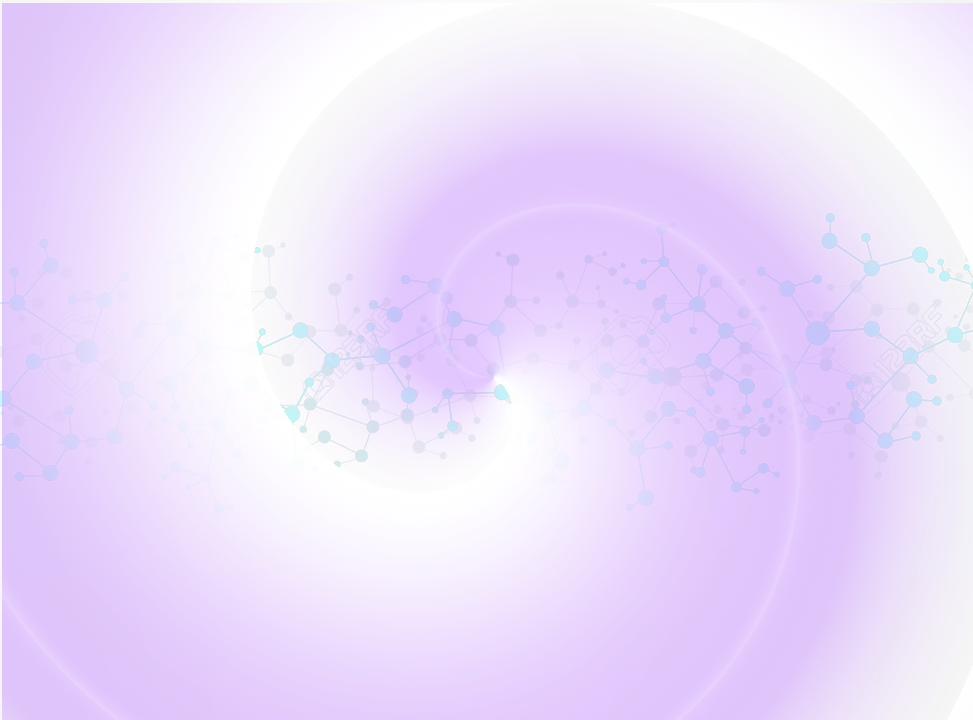
\includegraphics[width=\paperwidth,height=\paperheight]{uspex2}%
}
%---------------------------------------------------------------------------------
\title{
استفاده از Beamer برای تهیه اسلاید پارسی
}
\subtitle{ساخت اسلاید با زی‌پرشین و بیمر به روش ساده‌}
\author[مرصاد مستقیمی]{مرصاد مستقیمی
\\[.1cm]
 استاد راهنما: دکتر محمود اشرفی زاده
}
\institute[صنعتی اصفهان]{دانشگاه: صنعتی اصفهان}
\date{\today}


\begin{document}
\begin{persian}
%------------------------------------------
% Title page
%------------------------------------------
% 
% {\nologo
\begin{frame}[plain,noframenumbering]
%برای عدم نمایش نوار بالایی و پایین در فرم آپشن plain و برای اینکه جزء شماره اسلاید محسوب نشود آپشن فرم noframenumbering قرار داده شده است.
% \centerline{
\includegraphics[width=\paperwidth,height=\paperheight]{besm2.jpg}}
%دو انتخاب برای بسم الله هر کدام را نمی خواهید کامنت و دیگری را فعال کنید
\centerline{
\includegraphics[width=0.99\paperwidth,height=0.99\paperheight]{besmellah}}
\end{frame}
%%%%%%%%%%%%%%
\begin{frame}

\begin{picture}(0,0)
\put (-300,-125){\centerline{
\includegraphics[width=1.9cm]{logo}}}
\end{picture}
\vskip 0.20 in
\maketitle
\end{frame}
% }
% \begin{frame}
% \maketitle
% \end{frame}

% To adjust the paragraphs in RTL
\everypar{\rightskip\rightmargin}
%-------------------------------------------------------------------------------
\begin{frame}{سرآغاز}
\section{مبانی}
\subsection{متن ساده}
این یک نمونه بسیار ساده از اسلاید است که با بیمر و زی‌پرشین ساخته شده‌است.

 درکل بلور گسترده‌اند\LTRfootnote{\citet{Marzari2012}}

از فونت آزاد Roya XB برای این اسلاید استفاده شده‌است. این فونت در اینترنت موجود است و باید روی کامپیوتر شما نصب شده باشد یا در فولدر قابل دسترس برای زی‌لاتک باشد

تنظیمات اندکی در بخش آغازین برای اصلاح لیست‌ها و عنوان اسلایدها اضافه شده است. همچنین نحوه شماره‌گذاری تصاویر و جدول‌ها تنظیم شده‌است.

بسیاری از تم‌های استاندارد بیمر با این الگو قابل استفاده است.

استفاده از پانویس توصیه نمی شود. سفارش می‌شود که جدول فهرست مطالب به شکل دستی باشد. این اسلاید با بسیاری از تم‌های بیمر کار میکند اگرچه ممکن است اشکالاتی وجود داشته باشد.
\end{frame}

%-------------------------------------------------------------------------------
\section{لیست‌های بدون شماره و با شماره}
%-------------------------------------------------------------------------------
\begin{frame}{استفاده از لیست‌های بدون شماره}

استفاده از محیط لیست‌های بدون شماره در این‌جا آورده شده است. به نحوه راست چین نمودن لیست در فایل tex دقت نمایید.
\begin{itemize}\RTList
	\item مورد اول
	\item مورد دوم
	\item مورد سوم که یک متن طولانی تر است\\ ما چند خط در اینجا آورده‌ایم
	\item مورد آخر
\end{itemize}
\end{frame}

%-------------------------------------------------------------------------------
\begin{frame}{استفاده از محیط شماره‌گذاری}
 استفاده از محیط لیست (itemize) و شماره‌گذاری (enumerate) بصورت ترکیبی در این‌جا آورده شده است
 \begin{enumerate}\RTList
      \item سطح یک - مورد اول
	      \begin{itemize}\RTList
	      		\item  سطح دوم - مورد اول
	     		 \item  سطح دوم - مورد دوم
	      \end{itemize}
      \item سطح یک - مورد دو
      \item سطح یک - مورد سه
 \end{enumerate}

این یک پاراگراف ساده پارسی بعد از محیط شماره‌گذاری است.
\end{frame}


%-------------------------------------------------------------------------------
\begin{frame}{استفاده از رنگ و متن انگلیسی در اسلاید پارسی}
در این اسلاید نحوه استفاده از رنگ از بسته xecolor و نیز محیط LTR برای نوشتن متن پارسی آمده‌است.
\vspace{1cm}

{\xecolor{green}
	استفاده از \textbf{رنگ} و متن انگلیسی در داخل اسلاید پارسی
}
\vspace{1cm}
{\xecolor{red}
	\begin{LTR}
		This is an English Paragraph inside a Persian slide!\\
		Another line of latin text.
	\end{LTR}
}

\end{frame}


%-------------------------------------------------------------------------------
\begin{frame}
\frametitle{معادلات ریاضی}
چنانکه ملاحظه می‌شود عنوان در بیمر + زی‌پرشین به درستی کار می‌کند
\vspace{2cm}
\begin{equation}
\int_{a}^{b} f(x)dx = \frac{\lambda x^2 + \gamma x + \beta}{1+\sum_{n=1}^{m+2} 3 \alpha x^2 +x_n \sin(2 x_n -1)}
\end{equation}

\end{frame}

%------------------------------------------
% Tables and Pictures
%------------------------------------------
\section{کار با تصویر و جدول}

%------------------------------------------
\begin{frame}
\frametitle{شکل‌ها}
\begin{figure}
	\centering
	
\includegraphics[width=0.4\linewidth]{settings-blue.pdf}
	\caption[نمونه تصویر]{چگونگی درج یک تصور در بیمر+زی‌پرشین}
	\label{fig:pic1}
\end{figure}
\end{frame}


%-------------------------------------------------------------------------------
\begin{frame}{جداول در بیمر و زی‌پرشین}
\begin{table}
\caption{نمونه متن در جدول فارسی}
\begin{tabular}{|c|c|c|c|}
	\hline 
خانه اول	& خانه وسط جدول &خانه سمت راست    \\ 
	\hline 
ردیف دوم	&  ردیف دوم خانه دوم& ردیف دوم خانه سوم   \\ 
	\hline 
ردیف سوم	&
$ y=\int_{a}^{b\gamma+\epsilon} f(x) dx $
& ردیف سوم آخر   \\ 
	\hline 
\end{tabular} 
\end{table}
\end{frame}

%-------------------------------------------------------------------------------
\begin{frame}{اسلاید پایانی}
در نسخه بعدی این اسلاید موارد زیر  آمده‌است: استفاده از فونت‌های فارسی آزاد که مناسب اسلاید هستند، متن‌های چند ستونی، لیست‌های رنگی و ...

کد منبع این اسلاید در آدرس زیر موجود است
\begin{itemize}\RTList
	\item \href{https://github.com/kookma/Persian-Beamer-Templates}{Github/kookma}
\end{itemize}

\begin{alertblock}{نکته مهم}
	این اسلاید با انجام برخی تنظیمات تهیه شده است زیرا بسته زی‌پرشین هنوز بطور کامل با بیمر سازگار نیست. در سایت 
	\href{http://qa.parsilatex.com}{پرسش و پاسخ پارسی لاتک}
 روش‌های سیستماتیک و مناسب‌تری توسط توسعه دهنده زی‌پرشین ارایه شده‌است.
\end{alertblock}


\end{frame}
\begin{frame}{مراجع}
\footnotesize
\renewcommand\refname{}
\renewcommand{\addcontentsline}[3]{}% Remove functionality of \addcontentsline
\renewcommand{\section}[2]{}% Remove functionality of \section
 \begin{latin}
\bibliography{./chapters/bib}
\end{latin}
\end{frame}
\end{persian}
\end{document}
